\documentclass[./00PhotoBox.tex]{subfiles}
\graphicspath{{\subfix{./img/}}}

\begin{document}

\chapter{Bedienungsanleitung}

\section{Zweck}
Ziel des Systemes ist es, 3D-Modelle von Objekten bis zu einer Größe von 40~cm Durchmesser zu erstellen. Die Bedienung soll dabei möglichst einfach und selbsterklärend sein, um auch Laien die Möglichkeit zu geben, das System zu bedienen.

\section{Inbetriebnahme}
Beim Aufstellen ist darauf zu achten, dass sich keine stärkeren seitlichen Lichtquellen um das System herum befinden, wie beispielsweise auch Fensterflächen. Diese könnten die Belichtung der Bilder beeinflussen und so die Qualität der 3D-Modelle negativ beeinflussen. Gegebenenfalls muss für Verschattung oder Streuung gesorgt werden.

Die Berechnung des 3D-Modelles erfolgt auf einem externen Rechner. Hier kann wahlweise Agisoft Metashape oder OpenDroneMap (NodeODM) genutzt werden. Die entsprechende Software sowie eine Java-Laufzeitumgebung müssen auf dem Rechner installiert sein und die Bilder müssen auf diesen übertragen werden. Die Übertragung kann automatisch über eine Netzwerkverbindungen oder manuell per USB-Stick erfolgen. Die mitgelieferte Verbindungssoftware muss auf dem Rechner gestartet sein (siehe \autoref{sec:SoftwareEinrichtung}).

Das System startet bei Anschluss an eine Stromversorgung selbstständig. Da die Gefahr besteht, dass die kamerasteuernden Raspberry Pi Zero Daten verlieren, wenn die Stromversorgung unterbrochen wird, sollte das System immer ordnungsgemäß heruntergefahren werden und auf eine zuverlässige Stromversorgung geachtet werden.
Das Abschalten erfolgt durch langes Drücken auf den roten Taster. Das System fährt dann selbstständig herunter - erkennbar an dem Erlöschen der LEDs der Raspberry Pi Zero und der Beleuchtung - und die Stromversorgung kann getrennt werden.

\section{Software-Einrichtung}
\label{sec:SoftwareEinrichtung}
Die Software zur Steuerung der Kameras und zur Übertragung der Bilder auf den Rechner ist in Java geschrieben. Sie kann unter Linux, Windows und MacOS genutzt werden. Auf dem Rechner muss entsprechend eine Java-Laufzeitumgebung installiert sein. Für die Nutzung von Metashape muss eine Lizenz vorhanden sein und neben der ausführbaren jar-Datei abgelegt werden. Für OpenDroneMap muss die Software in Form von NodeODM auf dem Rechner installiert sein. Die Verbindung zu einem Server ist nicht implementiert.

\section{Kalibrierung}
Die letzten Koordinaten der Passpunkte wird im System gespeichert - daher sollten diese möglichst nicht verändert werden. Falls diese dennoch verändert werden, kann das System einzelne Veränderungen berechnen und nutzen. Bei Änderung einer Vielzahl muss das System jedoch extern neu kalibriert werden, beispielsweise durch Bilder mit einer externen Kamera, wo durch dann die Koordinaten der Passpunkte neu bestimmt werden können.

Eine Kalibrierung mit Bordmitteln ist nicht möglich.

\section{Durchführung}
Das System wird gestartet in dem die Stromversorgung hergestellt wird. Die Kameras starten selbstständig und die Beleuchtung wird eingeschaltet. Nach kurzer Zeit sollten kurz alle LEDs grün leuchten. Falls nicht, sind einige Kameras nicht erreichbar. Problemlösungen werden im Kapitel \autoref{sec:Problembehandlung} behandelt.

Das Objekt wird mittig, ggf. auf einer Erhöhung im Rahmen positioniert.

Ab hier trennen sich die Wege je nach verwendeten System. Die Bildaufnahme erfolgt in allen Fällen durch kurzen Druck auf den grünen Taster.

\begin{figure}
    \centering
    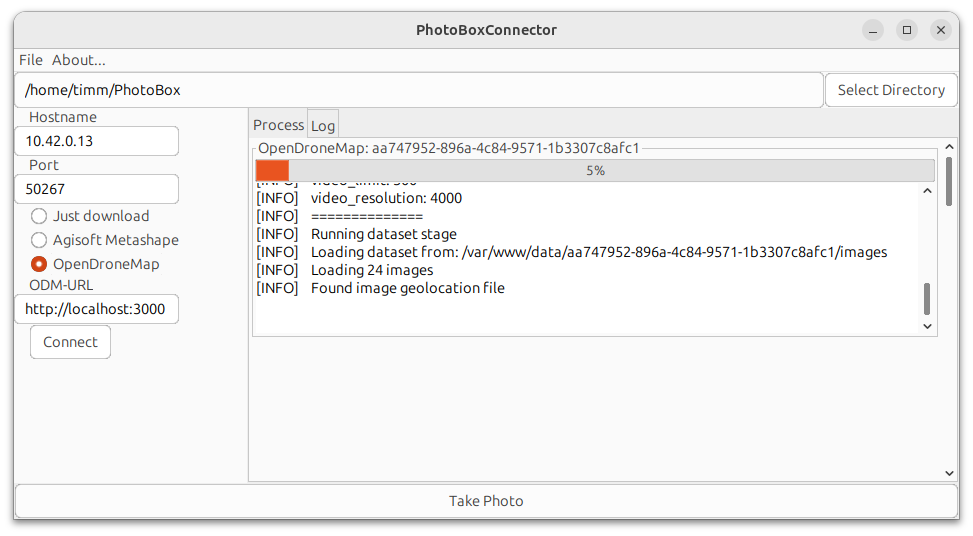
\includegraphics[width=1\textwidth]{./img/connector_screenshot.png}
    \centering
    \caption{Screenshot der Connector-Software unter Ubuntu 24.04} %Bildunterschrift
    \label{img:connector} %ID fürs Bild
\end{figure}

\subsection{mit Netzwerkverbindung}
Der zu verwendende Rechner wird mit dem System per WLAN (bevorzugt) oder Netzwerkkabel verbunden. Die Verbindungssoftware wird gestartet und die IP-Adresse des Systemes angegeben werden. Standardmäßig lautet diese im WLAN 10.0.1.1, per Netzwerkkabel muss die IP von einem DHCP-Server festgelegt werden, beispielsweise in dem der angeschlossene Rechner als DHCP-Server konfiguriert wird. Unter Gnome ist dieses beispielsweise möglich, indem in den Netzwerkeinstellungen die Internetverbindung des PC freigegeben wird.

Anschließend wird die zu nutzende Software ausgewählt und die Verbindung hergestellt.

Nun können die Bilder aufgenommen werden (grüne Taste). Die Bilder werden auf den Rechner übertragen und dort in der ausgewählten Software weiterverarbeitet. Der Fortschritt ist in der rechten Hälfte der Verbindungssoftware zu erkennen.

\section{Durchführung ohne direkte Weiterverarbeitung}
Alternativ können die Bilder auch ohne angeschlossenen PC aufgenommen werden und später weiter verarbeitet werden. Die Bilder werden in allen Fällen auf dem Raspberry Pi 4, der die gesamte Steuerung übernimmt, gespeichert. Die Bilder können dann von der Website des Raspberry Pi heruntergeladen werden. Auch ist es möglich, einen USB-Stick in den USB-Port des Raspberry Pi 4 vor der Bildaufnahme zu stecken. Die Bilder werden dann auch auf den USB-Stick kopiert.

Die Verbindungssoftware unterstützt auch das Laden der Bilder aus einem lokalen Ordner, beispielsweise aus der ZIP der Website oder dem Ordner auf dem USB-Stick.

\section{Wartung}
Software-Updates können zu Inkompatibilitäten führen, daher sollten diese erstmal auf einem zusätzlichen Raspberry Pi ausprobiert werden, bevor diese auf dem System ausgerollt werden.

\section{Fehlerbehebung}
\label{sec:Problembehandlung}
\subsection{Kameras sind nicht erreichbar}
Die Kameras sind nicht erreichbar, wenn die LEDs nicht grün leuchten. Dies kann verschiedene Ursachen haben. Als erstes sollte das System nochmal heruntergefahren werden durch einen langen Druck auf die rote Taste. Anschließend wird die Stromversorgung für einige Sekunden vollständig getrennt und wieder hergestellt. Das System sollte nun neu starten und die Kameras erreichbar sein.

Falls das noch nicht der Fall ist, hilft ein Blick in das Menü des WLAN-Routers. Hier sollten in der Übersicht aller Netzwerkgeräte die 24 Kameras, der steuernde Raspberry Pi 4 und das Gerät, über das der Zugriff erfolgt, aufgezählt sein. Falls das nicht der Fall ist, muss der fehlerhafte Raspberry Pi Zero an einen Display und eine Tastatur angeschlossen werden, um den Fehler zu finden.

Falls der Raspberry Pi im Netzwerk zu finden ist, kann sich per SSH mit dem Raspberry Pi verbunden werden. Zugangsdaten sind die Übersicht am Ende zu entnehmen.

\section{Zugangsdaten}

\begin{tabular}{|l|l|l|l|}
    \hline
    \textbf{Gerät}    & \textbf{Zugang} & \textbf{Benutzer} & \textbf{Passwort} \\
    \hline
    WLAN-Netzwerk     & photobox        &                   & photogrammetry    \\
    \hline
    Raspberry Pi 4    & 10.0.1.1        & photo             & box               \\
    \hline
    Raspberry Pi Zero & 10.0.2.1-24     & photo             & box               \\
    \hline
    WLAN-Router       & 10.0.0.1        &                   & photobox1         \\
    \hline
\end{tabular}

%\biblio
\end{document}